\begin{table}[htbp]
\centering
\small
\begin{tabular}{lcccc}
\multicolumn{5}{c}{\textbf{Illustrative External Cases Selected by Input--Output SSIM}} \\[3pt]
\hline
\textbf{Group} & \textbf{Case} & \textbf{SSIM} & \textbf{PSNR (dB)} & \textbf{MAE (HU)} \\
\hline
Least changed & Case 003 & $0.9809$ & $41.19$ & $8.76$ \\
 & Case 002 & $0.9756$ & $42.35$ & $8.10$ \\
 & Case 012 & $0.9586$ & $37.91$ & $9.64$ \\
Most changed & Case 015 & $0.7278$ & $23.32$ & $43.10$ \\
 & Case 005 & $0.7770$ & $20.77$ & $63.90$ \\
 & Case 008 & $0.8334$ & $33.53$ & $20.39$ \\
\hline
\end{tabular}
\par\smallskip\footnotesize Cases were selected only by the extremes of SSIM(Input, Output). High SSIM denotes less structural change between input and output; this ranking does not define artifact-removal quality or clinical acceptability.
\captionsetup{skip=2pt}
\caption[Illustrative external cases by input-output SSIM]{Descriptive external cases with the highest and lowest input--output SSIM values.}
\label{tab:external-ssim-extremes}
\end{table}

\begingroup
\setlength{\intextsep}{4pt}
\begin{figure}[H]
\centering
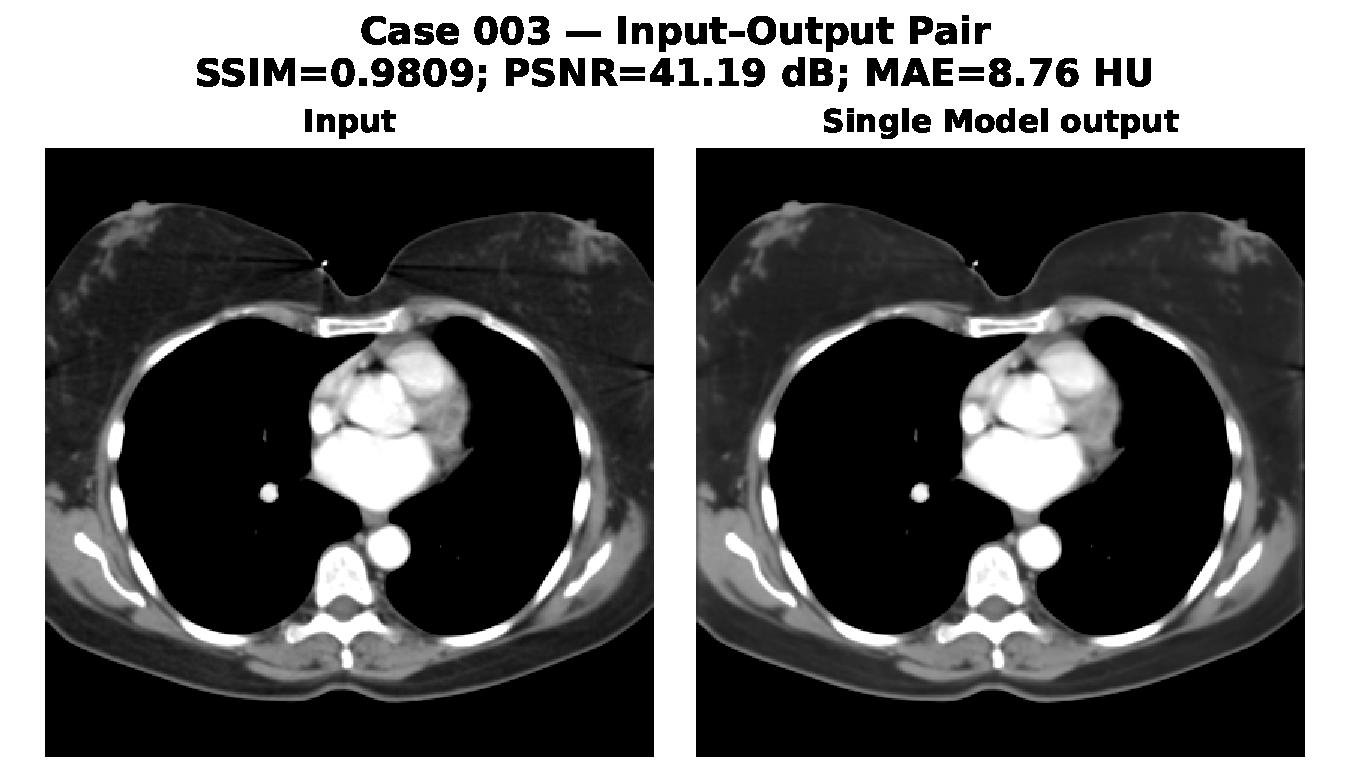
\includegraphics[width=0.84\linewidth]{Figures/Generated/external_evaluation/external_least_structurally_changed_case_003.pdf}
\end{figure}

\begin{figure}[H]
\centering
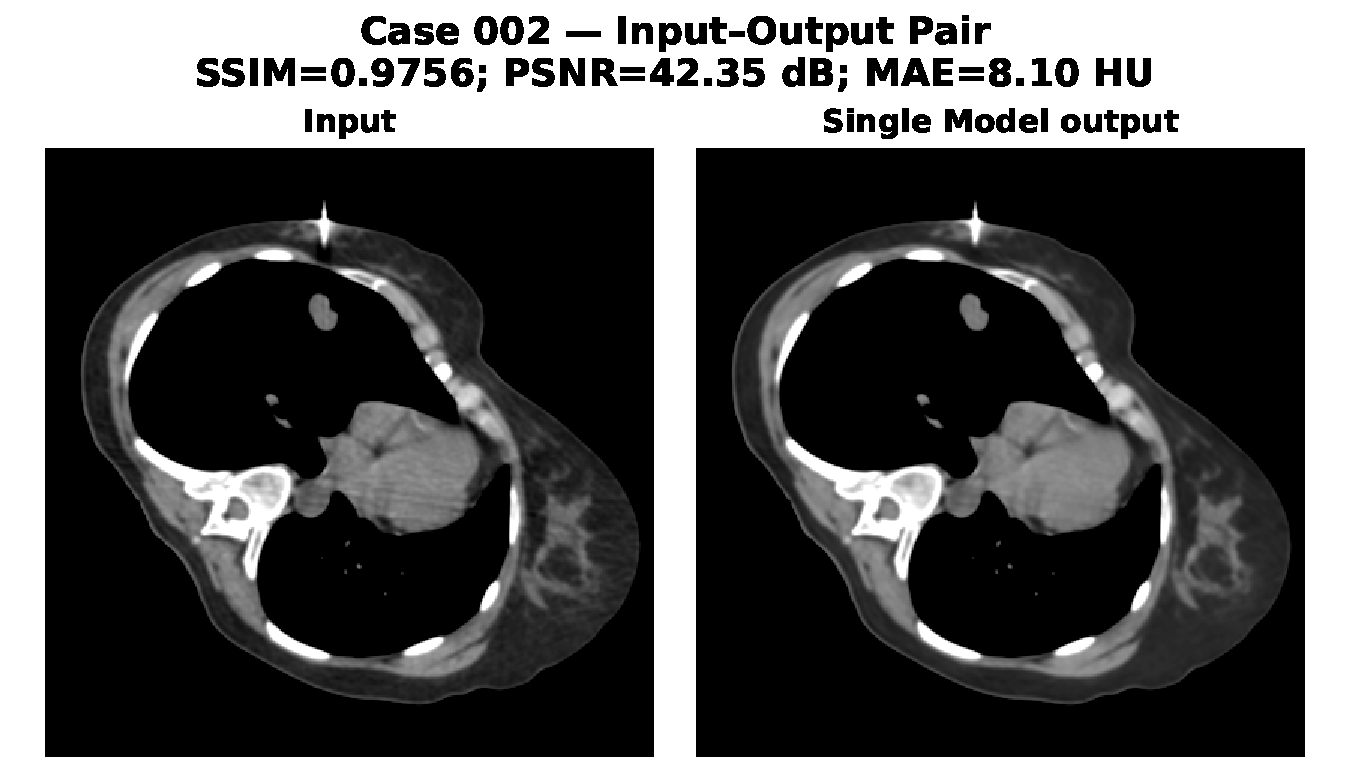
\includegraphics[width=0.84\linewidth]{Figures/Generated/external_evaluation/external_least_structurally_changed_case_002.pdf}
\end{figure}

\begin{figure}[H]
\centering
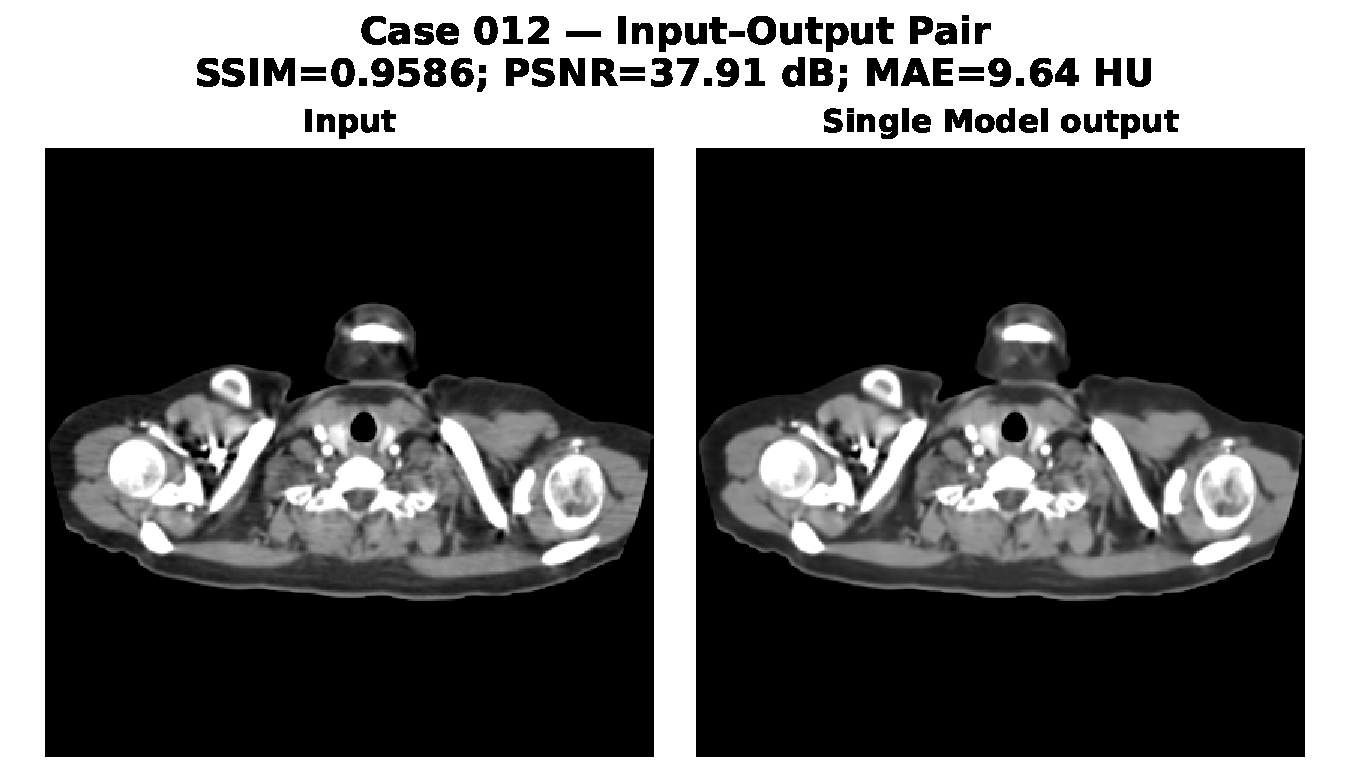
\includegraphics[width=0.84\linewidth]{Figures/Generated/external_evaluation/external_least_structurally_changed_case_012.pdf}
\end{figure}
\captionsetup{skip=1.5pt}
\captionof{figure}[Least structurally changed external cases]{External input-output pairs with the three highest SSIM values, representing the least structural change. The soft-tissue window is identical for input and output within each case.}
\label{fig:external-least-structurally-changed}
\endgroup

\begingroup
\setlength{\intextsep}{4pt}
\begin{figure}[H]
\centering
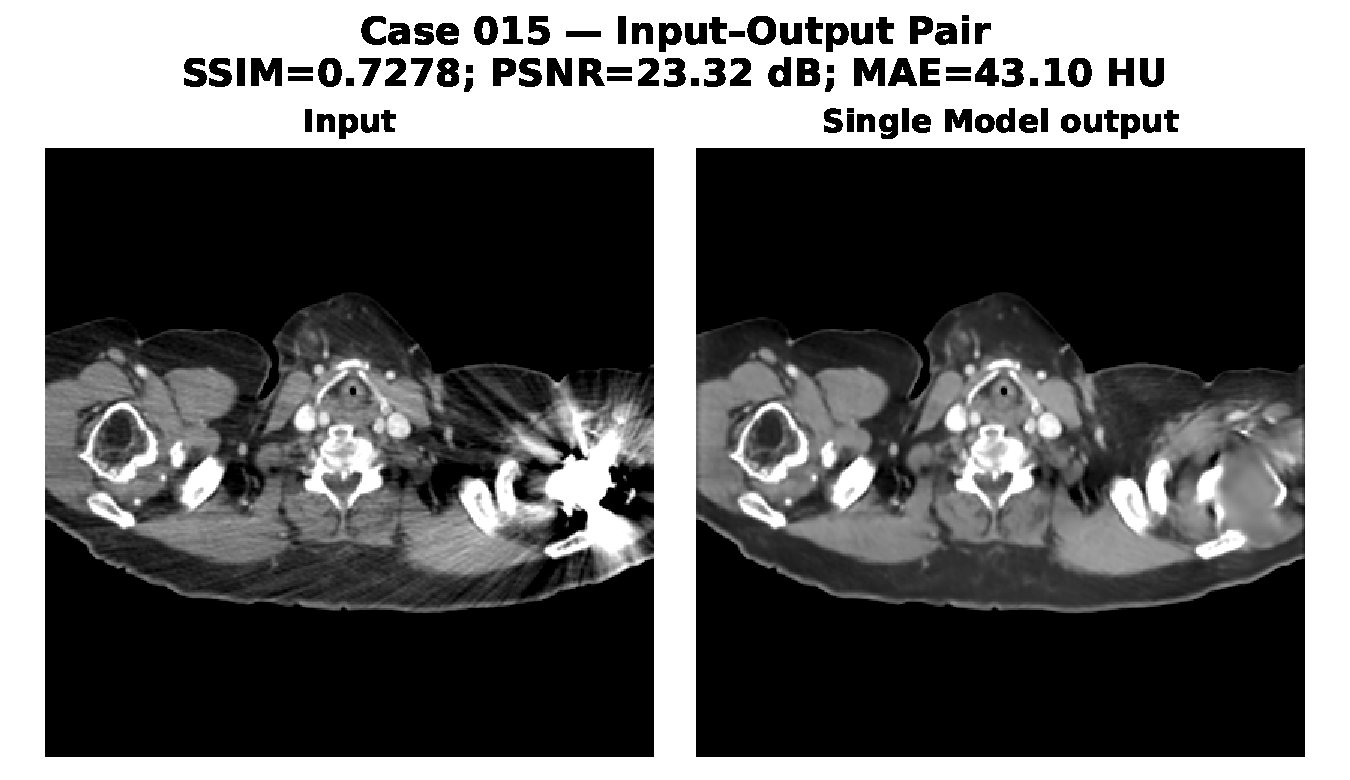
\includegraphics[width=0.84\linewidth]{Figures/Generated/external_evaluation/external_most_structurally_changed_case_015.pdf}
\end{figure}

\begin{figure}[H]
\centering
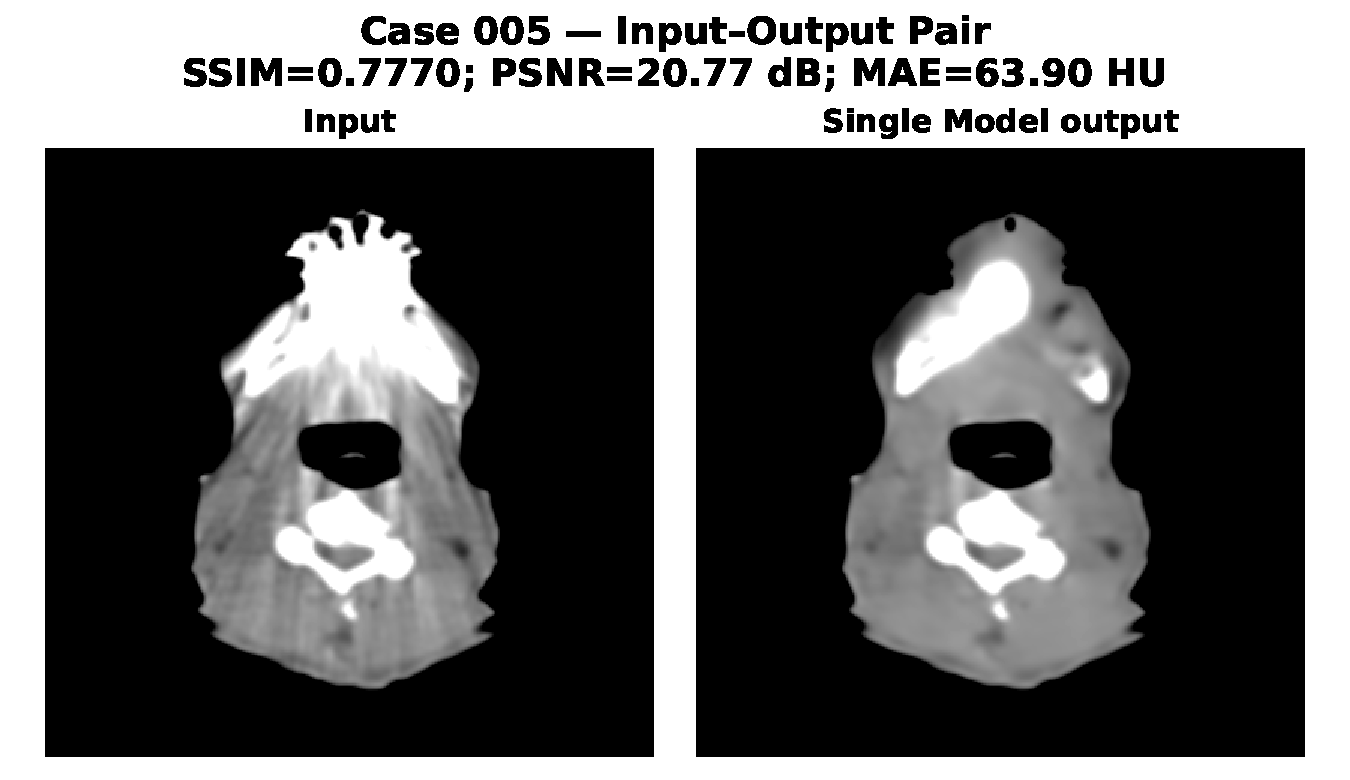
\includegraphics[width=0.84\linewidth]{Figures/Generated/external_evaluation/external_most_structurally_changed_case_005.pdf}
\end{figure}

\begin{figure}[H]
\centering
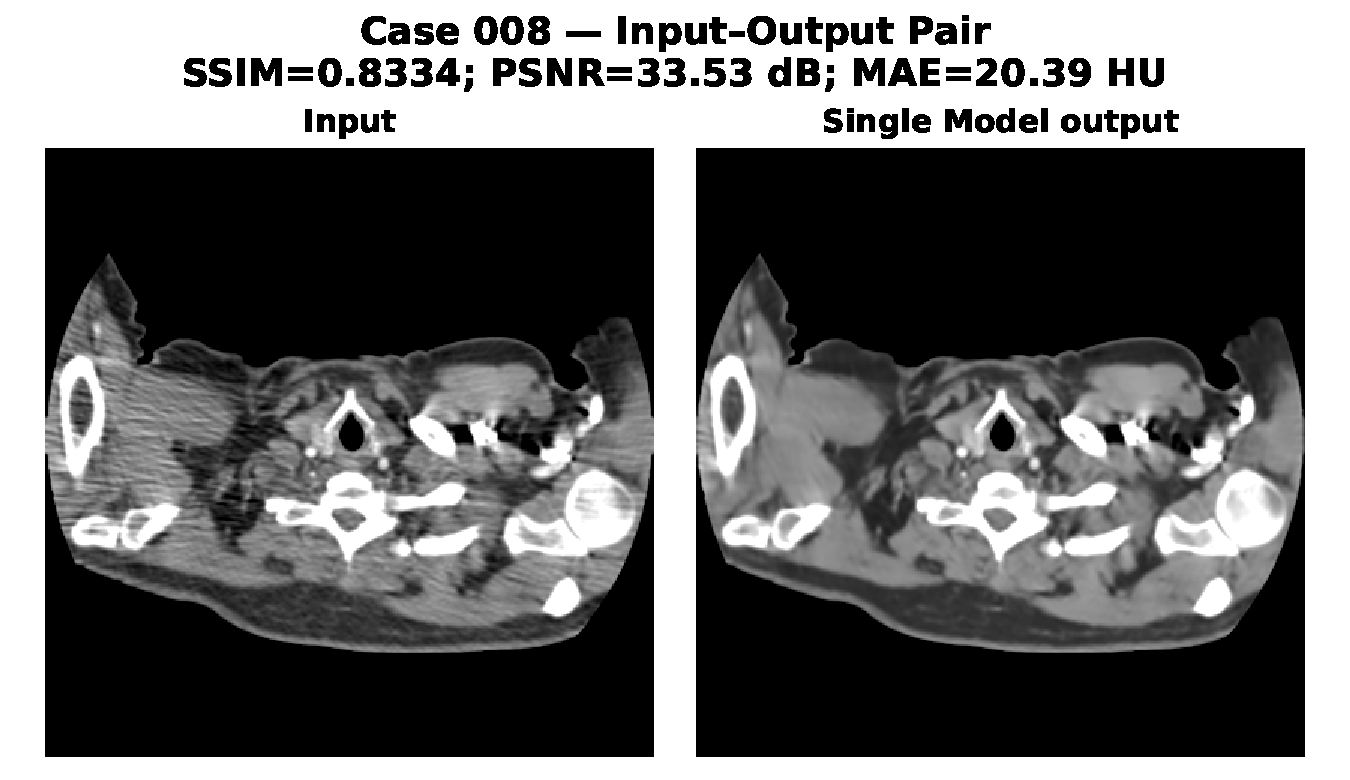
\includegraphics[width=0.84\linewidth]{Figures/Generated/external_evaluation/external_most_structurally_changed_case_008.pdf}
\end{figure}
\captionsetup{skip=1.5pt}
\captionof{figure}[Most structurally changed external cases]{External input-output pairs with the three lowest SSIM values, representing the greatest structural change. The soft-tissue window is identical for input and output within each case.}
\label{fig:external-most-structurally-changed}
\endgroup
